
\subsection{Описание блока формулирования задачи и рамочных требований к вводимым данным}
\label{sec:task_intro}

Сложность природных, антропогенных и экономических систем, участвующих в формировании морских прибрежных территорий, позволяет сделать вывод о невозможности формулирования единственного и универсального показателя, описывающего степень их удобства и пригодности к освоению.
Естественное многообразие сценариев использования прибрежных территорий определяет необходимость предусмотрения возможности реализации различных сценариев расчета и анализа, применимых к частным случаям и задачам городского планирования. 
Выбор типа такой задачи определяется предметной областью исследования, исходя из чего может быть делегирован пользователю методики.

В рамках поставленной цели исследования необходимыми условиями для решения любой подзадачи является исследумая береговая линия. \label{text:line_prop}
Допуская при этом, что решение части потенциальных задач предполагает выполнение расчетов для перспективных и проектируемых объектов рассматриваемый блок методики должен предусматривать возможность получения от пользователя исходной полилинии или набора точек, для которых будет выполняться анализ.
При этом определим обязательным условием то, что как исследуемая линия, так и точки должны принадлежать водному объекту или существующей береговой линии (не находиться на суше).

\begin{landscape}
	\begin{figure}
		\begin{center}
		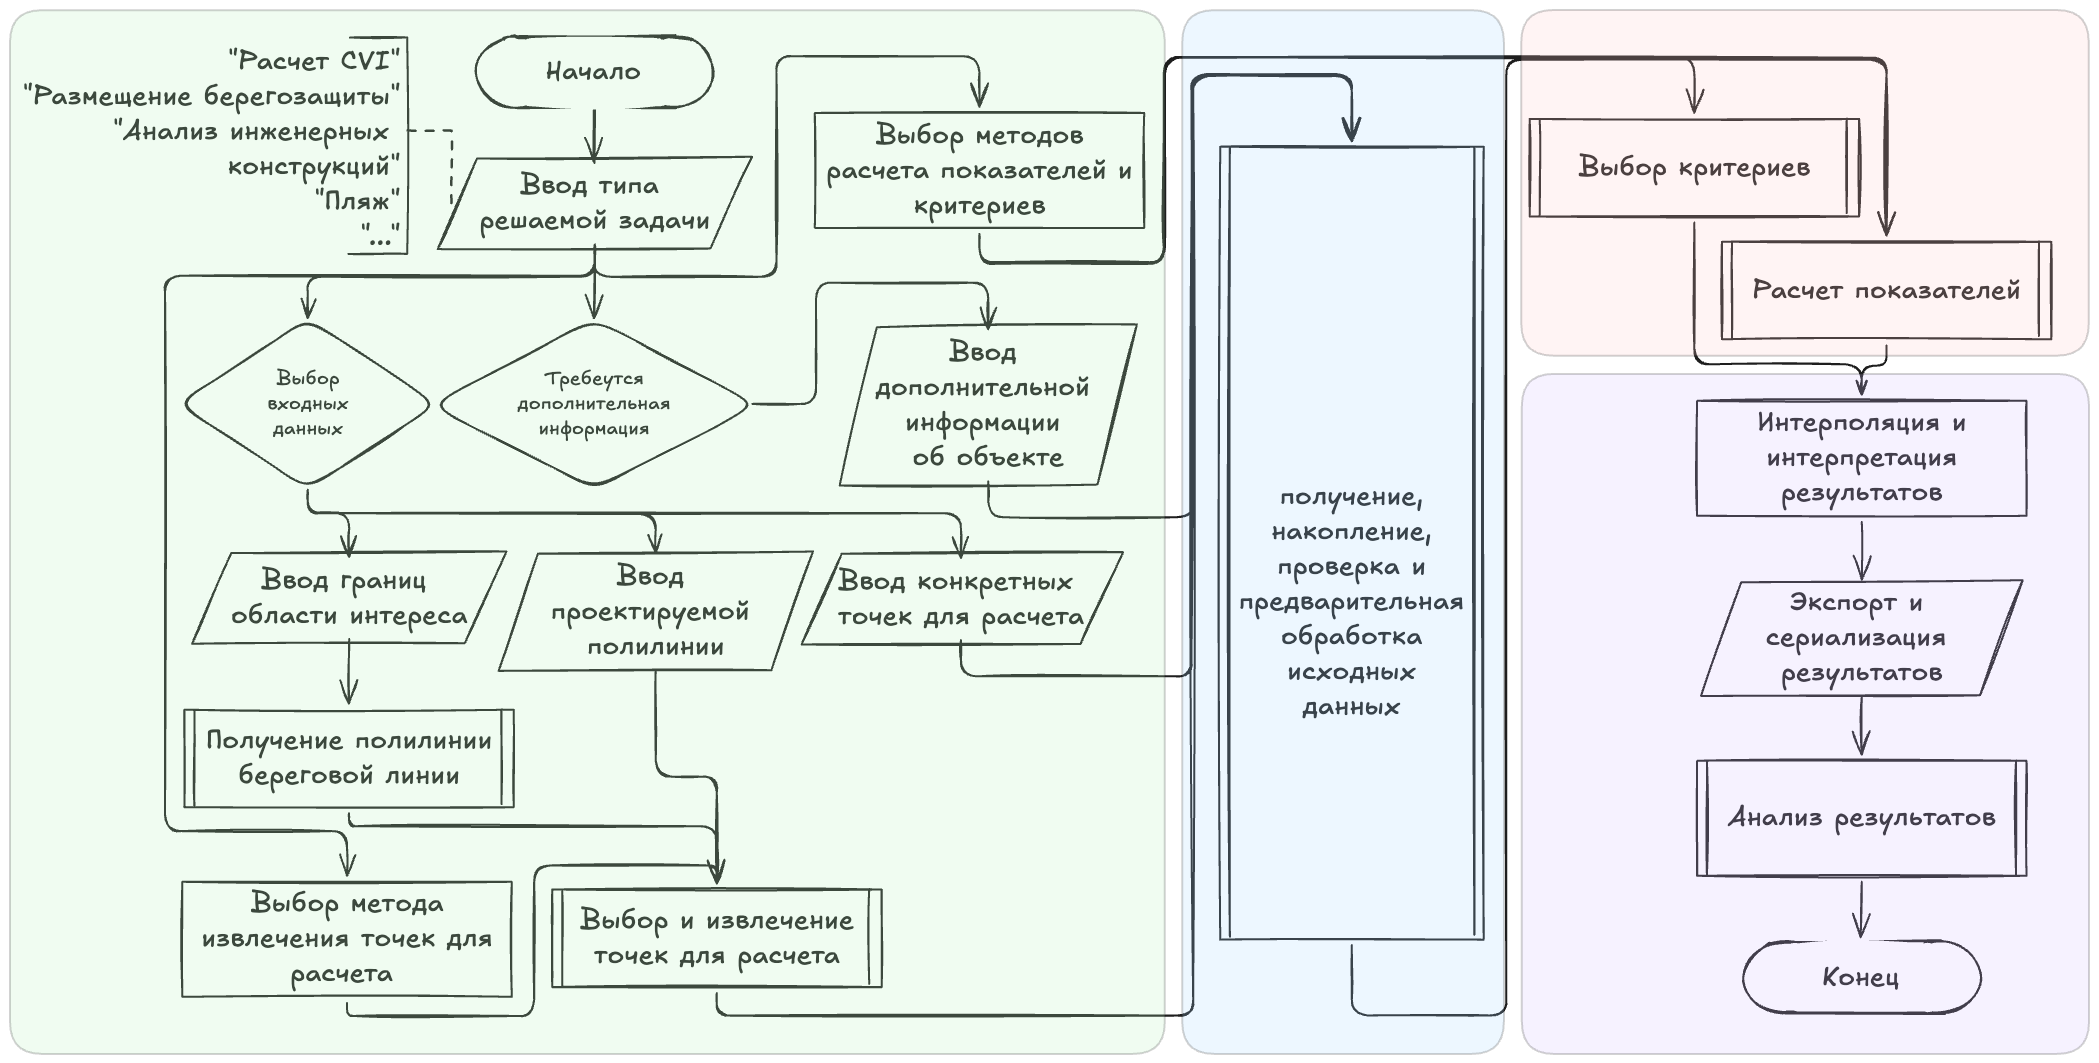
\includegraphics[width=\linewidth]{fig/part_2/БС_методики_v2.png}
		\caption{-- Блок схема алгоритма формирования задания}
		\label{pic:БС_формулирования_задачи}
		\end{center}
	\end{figure}
\end{landscape}

Обобщить описанные этапы выполнения блока формирования задания в общем процессе методики можно в виде блок-схемы, представленной на рисунке \ref{pic:БС_формулирования_задачи}. 

Следуя представленной схеме, на первом этапе пользователь выбирает конкретный тип задачи из списка реализованных методов оценки береговой линии.
Конкретный метод расчета при этом определяет тип и объем необходимых к вводу исходных данных.

Так, в случае решения крупномасштабных задач, например, при общем анализе береговой линии, достаточно задать лишь границы области интереса после чего должен отработать субпроцесс по извлечению береговой линии из источников открытых данных (описанных далее в разделе~\ref{sec:coastline_tools} на стр.~\pageref{sec:coastline_tools}).
Так как автоматический процесс извлечения данных может допускать присутствие \enquote{мусорных} объектов этот субпроцес может опционально дополняться операциями проверки, фильтрации и упрощения трассы береговой линии (описаными в разделе~\ref{sec:main_line_bulding} на стр.~\pageref{sec:main_line_bulding}).

В случае, если реализуемые алгоритмы автоматического извлечения береговой линии не удовлетворяют требованиям пользователя, или решаемой им задачи, загрузка необходимых данных о положении береговой линии может быть выполнена из отдельного предварительно созданного файла.
При этом базовыми форматами для загрузки являются общераспространенные ГИС форматы (\texttt{GeoJSON}, \texttt{GeoPackage} и~т.\,п.) или CAD форматы (при условии сохранения требуемой географической системы координат).

Опираясь на конкретный тип решаемой задачи, далее запускается процедура выбора метода отбора и извлечения точек, участвующих в последующем анализе.
В случае, если реализованные процедуры отбора точек для расчета не удовлетворяют частично или полностью требованиям решаемой задачи, у пользователя остается возможность загрузки файла с набором точек, для которых необходимо выполнить расчет как совместно с автоматически выбранными точками, так и отдельно от них.
Требования к формату вводимых пользователем данных эквивалентно к требованиям наложенным ранее на полилинии.

В результате у нас есть набор точек, принадлежащих некому линейному объекту, разделяющему водный объект и сушу.
Опираясь на то, что дальнейшие вычисления будут выполняться циклично для каждой точки из набора, рассмотрим все дальнейшие операции применительно к отдельной точки $M(x_0,y_0)$.
Что мы теряем при этом?
Сузив фокус внимания до отдельной точки, мы сохраняем знание лишь о ее положении, утрачивая информацию о линии в целом, положении смежных точек, а так же о размещении относительно нее водного объекта и суши.

Компенсировать эту утрату можно, сопоставив точку $M$ собственным вектором нормали $\vec{n}=(A,B)$, определяющим прямую перпендикулярную береговой линии и проходящим через точку $M$.
Для удобства дальнейших вычислений будем считать, что положительное направление вектора $\vec{n}$ выбрано так, что море располагается по сторону положительных значений линейной формы:
\begin{equation}\label{eq:norm_vect_line}
F(x,y) = A(x - x_0)+B(y - y_0).
\end{equation}

То есть для любой точки $(x,y)$, принадлежащей морю, выполняется $F(x,y)>0$.

Приведенного математического описания достаточно для локального описания береговой линии в области точки $M$, и понимания как относительно нее расположены море и суша.

Ранее, в разделе~\ref{part:methods_intro}, были приведены примеры, когда в условиях частных случаев некоторых задач требуются различные методы учета влияния на береговую линию определяющих ее сущностей.
Так как различные подтипы решаемых задач могут требовать для своей реализации специфичных исходных данных, автоматизировать процесс сбора которых не всегда возможно.
В связи с этим, в рамках рассматриваемого этапа, от пользователя могут быть дополнительно получены необходимые специфичные исходные данные, которые будут переданы на следующие этапы расчетов.

\label{sec:task_end}
В итоге, результатом работы блока формулирования задания будет являться экземпляр класса \enquote{задания}, обладающий единым интерфейсом, позволяющим на последующих этапах расчета гарантировано обеспечить консистентность выполнения следующих блоков алгоритма и обеспечить их всей необходимой информацией об анализируемом объекте.

% ===

% Не смотря на важность формализации задания, весьма вероятно, что используемые на этом этапе методы будут обращаться у известным методам и алгоритмам обработки геопространственных данных и не должны создавать значимых трудностей в ходе своей реализации на ровне с блоком экспорта.
